\PassOptionsToPackage{ukrainian,english}{babel}
\documentclass[twocolumn]{el-author}

%\usepackage[...]{...}      This has been commented out as we are not using any additional packages here.  On the whole, they should be unnecessary.
\usepackage{mathtext}
\usepackage[T1,T2A]{fontenc}
\usepackage[english,ukrainian]{babel}
\usepackage{hyperref}
\usepackage{graphicx} %package to manage images
\usepackage[a4paper, total={7in, 9.5in}]{geometry}
\usepackage{makecell}
\graphicspath{ {images/} }
\newcommand{\hH}{\hat{H}}
\newcommand{\D}{^\dagger}
\newcommand{\ua}{\uparrow}
\newcommand{\nc}{\newcommand}
\renewcommand\theadfont{\normalsize\scshape}
\nc{\da}{\downarrow} \nc{\hc}{\hat{c}} \nc{\hS}{\hat{S}}
\nc{\bra}{\langle} \nc{\ket}{\rangle} \nc{\eq}{equation (\ref}
\nc{\h}{\hat} \nc{\hT}{\h{T}}\nc{\be}{\begin{eqnarray}}
\nc{\ee}{\end{eqnarray}}\nc{\rd}{\textrm{d}}\nc{\e}{eqnarray}\nc{\hR}{\hat{R}}\nc{\Tr}{\mathrm{Tr}}
\nc{\tS}{\tilde{S}}\nc{\tr}{\mathrm{tr}}\nc{\8}{\infty}\nc{\lgs}{\bra\ua,\phi|}\nc{\rgs}{|\ua,\phi\ket}
\nc{\hU}{\hat{U}}\nc{\lfs}{\bra\phi|}\nc{\rfs}{|\phi\ket}\nc{\hZ}{\hat{Z}}\nc{\hd}{\hat{d}}\nc{\mD}{\mathcal{D}}
\nc{\bd}{\bar{d}}\nc{\bc}{\bar{c}}\nc{\mc}{\mathcal}\nc{\ea}{eqnarray}\nc{\mG}{\mathcal{G}}\nc{\bce}{\begin{center}}
\nc{\ece}{\end{center}}
\date{20 Грудня 2018}

\begin{document}

\title{Вивчення явища фотоефекту та визначення сталої Планка}

\author{Сергій Поліщук}

\abstract{Макс Планк ввів свою сталу для пояснення спектру випромінювання абсолютно чорного тіла, припустивши, що тіло випромінює електромагнітні хвилі порціями (квантами) з енергією, пропорційною частоті (hv). У 1905 році Ейнштейн використав це припущення для того, щоб пояснити явище фотоефекту, постулювавши, що електромагнітні хвилі поглинаються порціями з енергією пропорційною частоті. Так зародилася квантова механіка...}

\maketitle

\section{Мета роботи}

вивчення явища зовнішнього фотоефекту. 

\section{Прилади і матеріали}

лампа розжарювання з джерелом живлення,
фотопомножувач ФЕГІ-2 у світлонепроникному корпусі,
набір світлофільтрів, гальванометр, вольтметр, акумулятор.

\section{Завдання}

\begin{enumerate}
	\item при домашній підготовці:
	\begin{itemize}
		\item  засвоїти теоретичні відомості щодо визначення сталої
Планка;
		\item  зарисувати у робочий зошит електричну схему;
		\item  описати і будову та принцип дії приладів, щo використовуються.
	\end{itemize}
	\item при виконанні роботи:
	\begin{itemize}
		\item  скласти електричну схему і показати її викладачеві для перевірки;
		\item  визначити сталу Планка методом затримуючого потенціалу;
		\item  виконати необхідні розрахунки з визначення шуканої величини;
		\item  оформити звіт і подати його викладачеві.
	\end{itemize}
	
\end{enumerate}

\section{Правила техніки безпеки}

\begin{itemize}
	\item  розташуйте прилади таким чином, щоб уникнути їх падіння;
	\item  при складанні електричної схеми використовуйте провідники з непошкодженою ізоляцією.
\end{itemize}

\section{Теоретичні відомості та опис установки}

Під зовнішнім фотоефектом розуміють звільнення електронів з поверхні металів за допомогою світла. Явище було відкрите у 1887 році Г.~Герцем, а пояснене А.~Ейнштейном у 1905 році. Виходячи з квантових уявлень, Ейнштейн закон збереження енергії при взаємодії кванта світла йиз електроном речовини записав у вигляді формули, яка зараз носить його ім'я:

\begin{equation} \label{eq:Einstein}
hv = A+\frac{m_{e}V_{max}^{2}}{2}
\end{equation}

Тут $A$ - робота виходу електрона з металу, $m_{e}$ - маса електрона, $V_{max}$ - його максимальна швидкість.

Щоб припинити вихід електронів, потрібно прикласти до металу зворотну гальмівну різницю потенціалів, величина якої $U$ визначається із співвідношення:

\begin{equation} \label{eq:Einstein_reverse}
\frac{m_{e}V_{max}^{2}}{2} = eU
\end{equation}

У цьому разі $hv = A + eU$. Оскільки для даного металу $A = const$, то гальмівна напруга залежить лише від частоти му світла, яке спрямовується на метал. Це відкриває можливість, вимірявши гальмівні напруги $U_{1}$ і $U_{2}$ при освітленні фотоелемента світлом двох різних частот $v_{1}$ і $v_{2}$, визначити сталу Планка h:

\begin{equation} \label{eq:1}
\left\{\begin{matrix}
hv_{1} = A+eU_{1}
\\ hv_{2} = A+eU_{2}
\end{matrix}\right.
\end{equation}

Розв'язок цієї системи рівнянь відносно й приводить до результату:

\begin{equation} \label{eq:1_1}
h = \frac{e(U_{1} - U_{2})}{v_{1} - v_{2}}
\end{equation}

або через довжини світлових хвиль

\begin{equation} \label{eq:1_2}
h = \frac{e\lambda_{1} \lambda_{2}(U_{1} - U_{2}) }{c(\lambda_{1} - \lambda_{2})}
\end{equation}

Якщо скористатись принаймні трьома світлофільтрами із стандартного набору, то комбінуючи їх по два, можна одержати три результати відносно h, що є хоча і мінімальною, проте достатньою кількістю значень для визначення усередненої величини сталої Планка.

\begin{table}[ht]
\processtable{Спектральні характеристики деяких скляних світлофільтрів}
{\begin{tabular}{|l|l|l|l|l|}\hline
\thead{№} & 
\thead{{\scriptsize Марка} \\ {\scriptsize світлофільтра}} & 
\thead{{\scriptsize Товщина} \\ {\scriptsize скла, мм}} & 
\thead{{\scriptsize Довжина хвилі} \\ {\scriptsize максимального} \\ {\scriptsize пропускання, м}} & 
\thead{{\scriptsize Частота хвилі} \\ {\scriptsize максимального} \\ {\scriptsize пропускання, Гц}}\\\hline
1 & КС-13 & 2,78 & $700*10^{-9}$ & $4.3*10^{14}$ \\\hline
2 & OC-13 & 3,02 & $650*10^{-9}$ & $4.6*10^{14}$ \\\hline
3 & ЖС-18 & 3,07 & $600*10^{-9}$ & $5.0*10^{14}$ \\\hline
4 & 3C-1 & 1,00 & $540*10^{-9}$ & $506*10^{14}$ \\\hline
5 & CC-2 & 1,00 & $390*10^{-9}$ & $7.7*10^{14}$ \\\hline
6 & ФС-6 & 1,00 & $360*10^{-9}$ & $8.3*10^{14}$ \\\hline
\end{tabular}}{}
\end{table}

Інший шлях визначення сталої Планка, у межах цієї лабораторної роботи, наступний. З рівняння $hv = A + eU$ визначимо значення гальмівної напруги:

\begin{equation} \label{eq:2}
U = \frac{h}{e}v - \frac{A}{e}
\end{equation}

Звідси слідує, що залежність $U$ від частоти падаючого світла лінійна. Використавши шість вище зазначених світлофільтрів, одержимо шість значень для $U$. Графічно залежність $U$ від $v$ має вигляд відрізка прямої $BC$ на рис. \ref{img:1}

\begin{figure}[h]
\centering{\includegraphics[width=80mm]{img_1}}
\caption{\source{}}
\label{img:1}
\end{figure}

Провести цей відрізок слід так, щоб кількість точок, нанесених на
графік, зверху і знизу відрізка була однакова.

Із рівняння (\ref{eq:2}) слідує, що $tg\alpha = \frac{h}{e}$. Тоді,
визначивши із рис.\ref{img:1} $tg\alpha = \frac{U_{6} - U_{1}}{v_{6} - v_{1}}$, 
знаходимо $h = \frac{U_{6} - U_{1}}{v_{6} - v_{1}}\times e$. 
Тобто одержали, як і слід було чекати, той самий вираз, але графічним шляхом

\begin{figure}[h]
\centering{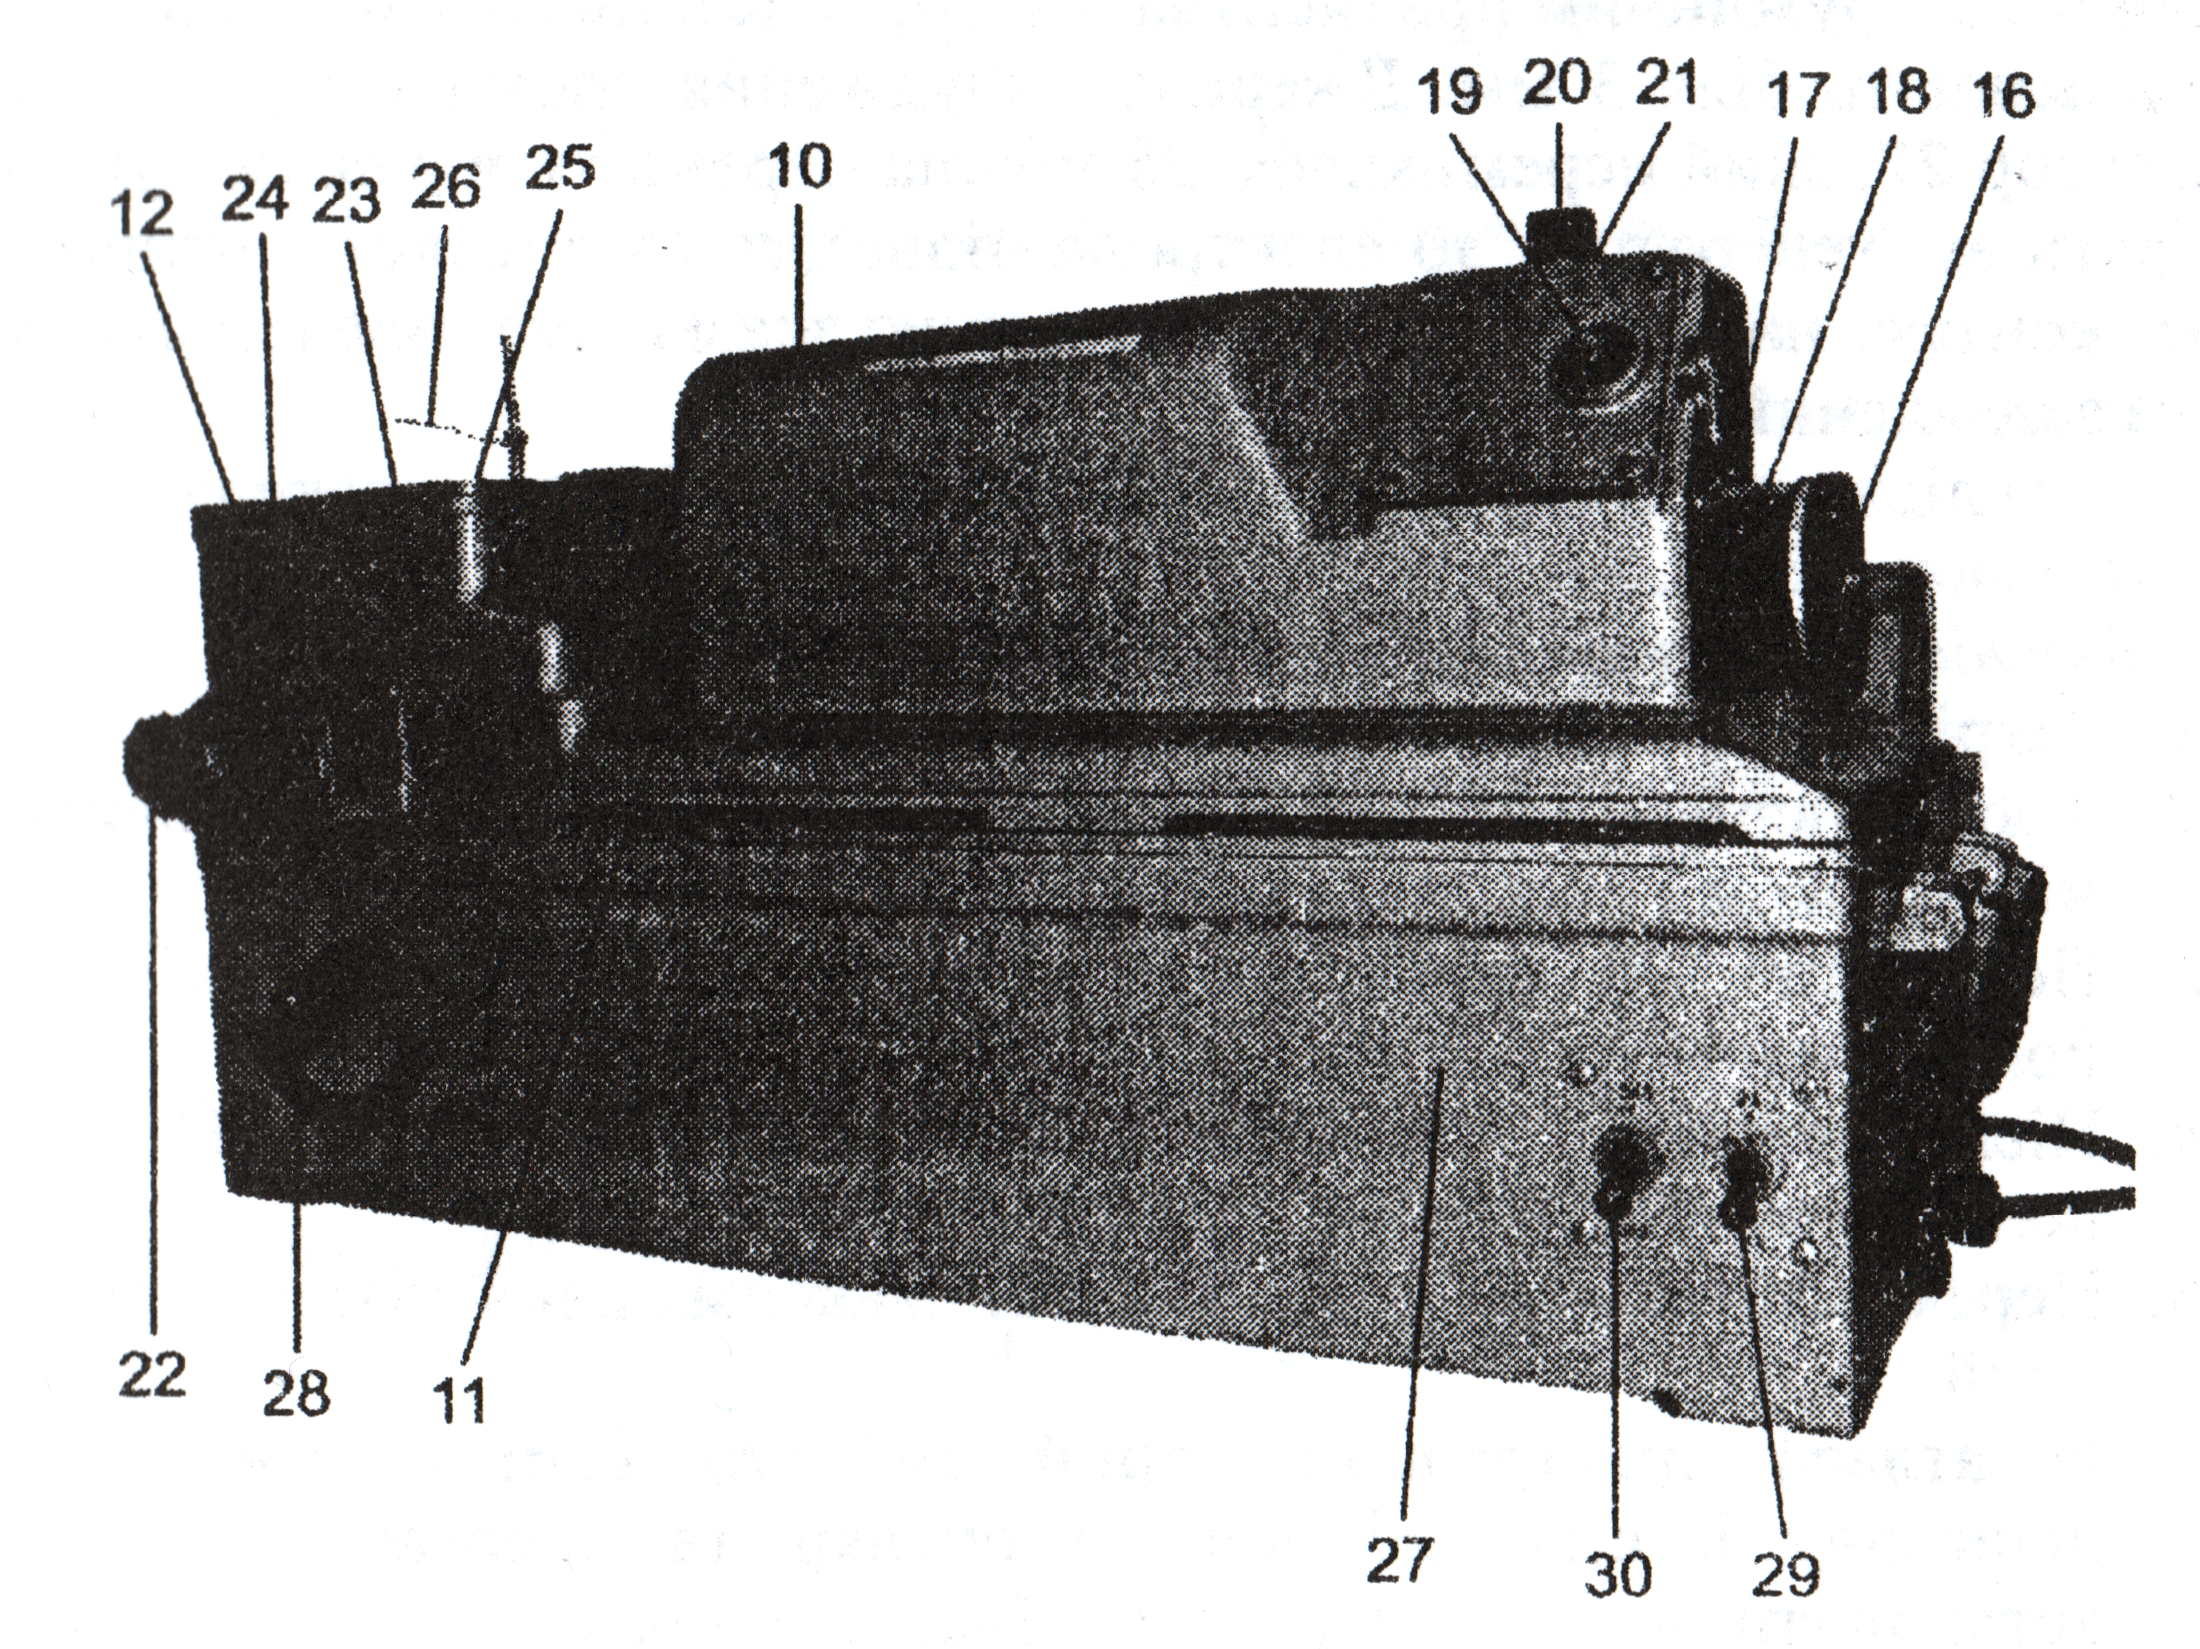
\includegraphics[width=80mm]{img_2}}
\caption{Вакуумний сурм'яно-цезієвий фотоелектронний помножувач ФЕП-2
\source{}}
\label{img:2}
\end{figure}

\begin{figure}[h]
\centering{\includegraphics[width=80mm]{img_3}}
\caption{\source{}}
\label{img:3}
\end{figure}

Продовживши відрізок $BC$ до перетину його з вертикальною віссю $U$,
отримуємо точку $D$. Із рівняння (\ref{eq:2}) слідує, що довжина відрізка $OD$, виміряна у масштабі напруг, дорівнює - $\frac{A}{e}$. Тоді:

\begin{equation} \label{eq:3}
A = e \times U_{r}
\end{equation}

Роботу виходу $A$ прийнято визначати у електрон-вольтах, вона для металів не перевищує кількох $еВ$.

У роботі використовується вакуумний сурм'яно-цезієвий фотоелектронний помножувач ФЕП-2. Його зовнішній вигляд зображено на puc.\ref{img:2}

Електрична схема установки складається з двох незалежних кіл - кола
освітлювача і кола фотопомножувача (рис. \ref{img:3}).

У якості освітлювача використовується низьковольтна лампочка
розжарення, яка живиться від випростувала ВС 4-12. Світло від лампочки
через світлофільтр спрямовується на фотопомножувач. Гальмівна напруга на
фотопомножувач подається через потенціометр від акумулятора. Вольтметр
повинен бути розрахований на декілька вольт і мати точність вимірювання не
гірше 0,1 В. Мікроамперметр необхідно вибрати якомога чутливим.

\section{Послідовність виконання роботи}

\begin{enumerate}
	\item Скласти електричну схему згідно рис. \ref{img:3}, 
		показати її для перевіркивикладачеві.
	\item Перед фотоелементом встановити світлофільтр.
	\item Тумблер на приладі ВС 4-12 поставити в положення «Вкл».
	\item Ключем К замкнути коло фотопомножувача.
	\item Спостерігаючи за показами  мікроамперметра, переміщувати
		повзунок реостату до положення, поки мікроамперметр локаже
		відсутність струму.
	\item Зняти з максимальною точністю покази вольтметра.
	\item Замінити світлофільтр. 
		\textit{Увага! При заміні світлофільтра слід
		обов'язково вимкнути освітлювач, перевівши тумблер на приладі
		ВС 4-12 у положення «Вик»},
	\item Після заміни світлофільтра повторити дії 3, 5, 6.
	\item Виміряти гальмівну напругу для усіх світлофільтрів.
	\item За формулою (\ref{eq:1_2}) визначити сталу Планка щонайменше для трьох
		пар світлофільтрів, розрахувати похибки вимірювань.
	\item Побудувати графік залежності гальмівної напруги від частоти
		падаючого на фотокатод світла.
	\item Користуючись одержаним графіком, визначити сталу Планка і
роботу виходу.
	\item Провести аналіз одержаних результатів, порівнявши їх з
табличними.
\end{enumerate}

\begin{thebibliography}{}

\bibitem{1}
Кучерук І.М., Горбачук І.Т. Загальний курс фізики: Т.3.: Оптика.
Квантова фізика. - К.: Техніка, 2006.- 518c., cr. 239 - 247.

\bibitem{2}
Кучерук ІМ, Дущенко В.П. Загальна фізика. Оптика. Квантова
фізика. - К.: Вища школа, 1999. -- 463с., ст. 260 - 264.

\bibitem{3}
орбачук ІТ. Загальна фізика. Лабораторний практикум. - К.:
Вища школа, 1992.- 512 с., ст. 434 - 437.

\bibitem{4}
Методична розробка до роботи.

\end{thebibliography}

\section{Завдання для самоконтролю}

\begin{enumerate}
	\item У чому полягає явище фотоефекту?
	\item Сформулюйте закони фотоефекту.
	\item Який вигляд має рівняння Ейнштейна для фотоефекту?
	\item Що таке робота виходу?
	\item Що таке червона межа фотоефекту?
	\item Яка будова вакуумного фотоелемента?
	\item Що таке затримуючий потенціал?
	\item Чим пояснити наявність струму насичення у вакуумних
		фотоелементів? Чи буде струм насичення у газонаповнених
		фотоелементів?
	\item Який принцип дії фотопомножувача?
	\item Чи існують явища обернені фотоефекту?
\end{enumerate}

\clearpage
\section{Тестові завдання для вхідного контролю}

\begin{enumerate}
	\item Під фотоефектом розуміють:
	\begin{enumerate}
		\item звільнення електронів з речовини при її освітленні;
		\item втрату металом позитивного заряду під дією світла;
		\item утворення в речовині під дією світла 
			пари «електрон-дірка»;
		\item перерозподіл у речовині під дією світла електронів 
			на енергетичних рівнях.
		\item перерозподіл у речовині під дією світла електронів 
			на енергетичних рівнях.
	\end{enumerate}
	Яке з цих тверджень є хибним?
	\item Яке з перелічених нижче явищ не може відбуватися під дією світла?
	\begin{enumerate}
		\item зовнішній фотоефект;
		\item ядерний фотоефект;
		\item внутрішній фотоефект;
		\item вентильний фотоефект.
	\end{enumerate}
	\item При фотоефекті проявляються:
	\begin{enumerate}
		\item хвильові властивості світла;
		\item корпускулярні властивості світла;
		\item дуалістичні властивості світла;
		\item дотепер невідомі властивості світла.
	\end{enumerate}
	\item Поверхня деякого тіла освітлюється світлом з частотою $v$. 
		Яку енергію може поглинати тіло?
	\begin{enumerate}
		\item $0.5 hv$
		\item $hv$
		\item $2 hv$
		\item будь-яку між $hv$ та $2 hv$
	\end{enumerate}
	\item Максимальна кінетична енергія вибитих світлом з 
		металу електронів не залежить від:
	\begin{enumerate}
		\item частоти падаючого світла;
		\item освітлюваного металу;
		\item інтенсивності світла;
		\item довжини світлової хвилі.
	\end{enumerate}
	\item Кількість електронів, вибитих світлом за 1 с з металу, залежить від:
	\begin{enumerate}
		\item освітлюваного металу;
		\item частоти світла;
		\item інтенсивності світла;
		\item температури металу.
	\end{enumerate}
	\item Фотоефект може припинитися, якщо:
	\begin{enumerate}
		\item збільшити в 2 рази температуру освітлювального металу;
		\item збільшити в 2 рази відстань між поверхнею металу і джерелом світла;
		\item зменшити в 2 рази світловий потік;
		\item зменшити в 2 рази частоту падаючого світла.
	\end{enumerate}
	\item Інерційність фотоефекта можна визначити за допомогою:
	\begin{enumerate}
		\item звичайного секундоміра;
		\item мікросекундоміра;
		\item мілісекундоміра;
		\item наносекундоміра.
	\end{enumerate}
	\item Падаюче на метал світло викликає фотоефект. 
	Якщо інтенсивність світлового потоку збільшити удвічі, 
	то кінетична енергія фотоелектронів:
	\begin{enumerate}
		\item не зміниться;
		\item збільшиться удвічі;
		\item збільшиться; 
		\item збільшиться учетверо.
	\end{enumerate}
	\smallskip
	\item Робота виходу електрона з металу:
	\begin{enumerate}
		\item $A = hv$;
		\item $A = \frac{hc}{\lambda_{min}}$
		\item $A = hv_{max}$
		\item $A = \frac{hc}{\lambda_{max}}$
	\end{enumerate}
\end{enumerate}

\newpage

\section{Тестові завдання для підсумкового контролю}

\begin{enumerate}
	\item Рівняння Ейнштейна для зовнішнього фотоефекту має вигляд:
	\begin{enumerate}
		\item $E = mc^{2}$
		\item $hv = A + \frac{mv^{2}}{2}$
		\item $\frac{mv^{2}}{2} = Q + hv$
		\item $A = \frac{mv^{2}}{2} + hv$
	\end{enumerate}
	\item Кількість електронів, вибитих світлом 
		з одиниці поверхні освітлюваного металу за 1 с, залежить від:
	\begin{enumerate}
		\item сили світла джерела;
		\item яскравості джерела світла;
		\item світлового потоку;
		\item освітленості поверхні металу.
	\end{enumerate}
	\item Яке(-і) твердження вірне(-і)? \\
		При фотоефекті кінетична енергія вибитих з металу 
		електронів залежить від:
	\begin{enumerate}
		\item частоти падаючого світла
		\item освітлюваного металу
		\item інтенсивності падаючого світла
	\end{enumerate}
	\item Довжина хвилі, що відповідає червоній межі фотоефекта:
	\begin{enumerate}
		\item $\lambda_{max} = \frac{A}{c}$;
		\item $\lambda_{max} = \frac{A}{h}$;
		\item $\lambda_{max} = \frac{hc}{A}$;
		\item $\lambda_{max} = \frac{Ac}{h}$
	\end{enumerate}
		де $A$ - робота виходу електрона з металу.
	\item При зовнішньому фотоефекті гальмівна напруга залежить:
	\begin{enumerate}
		\item лише від частоти світла;
		\item лише від інтенсивності світла;
		\item лише від того металу, який освітлюють;
		\item яквід металу, так і від частоти світла.
	\end{enumerate}
	\item Величина гальмівної напруги змінюється з частотою світла, 
		яке викликає фотоефект:
	\begin{enumerate}
		\item у прямій пропорційній залежності;
		\item у оберненій залежності;
		\item лінійно;
		\item за експоненціальним законом.
	\end{enumerate}
	\item На рисунку \ref{img:4} наведено графік залежності гальмівної напруги 
		від частоти світла, що діє на деякий метал. 
		Чи можна визначити за цим графіком який це метал?
		\begin{figure}[ht]
			\centering{\includegraphics[width=80mm]{img_4}}
			\caption{Графiк залежностi гальмiвної
напруги вiд частоти свiтла до завдання 7\source{}}
			\label{img:4}
		\end{figure}
	\begin{enumerate}
		\item не можна, недостатньо даних;
		\item це може бути платина;
		\item це срібло;
		\item це може бути цезій.
	\end{enumerate}
	\item Який з нижче наведених виразів для визначення 
		гальмівної напруги є принципово хибним?
	\begin{enumerate}
		\item $U = \frac{m_{e}V_{max}^{2}}{2e}$;
		\item $U = \frac{A}{e}$;
		\item $U = \frac{h}{e}v - \frac{A}{e}$;
		\item $U = \frac{h}{e}v$.
	\end{enumerate}
		де $m_{e}$ - маса електрона, $e$ - заряд електрона, $V$ - швидкість фотоелектрона, $A$ - робота виходу електрона з металу, $v$ - частота світла, що викликає фотоефект.
	\newpage
	\item Збільшення інтенсивності падаючого на метал світла призводить до:
	\begin{enumerate}
		\item збільшення кінетичної енергії вилітаючих електронів;
		\item збільшення фотоструму;
		\item збільшення гальмівної напруги;
		\item зменшення роботи виходу;
	\end{enumerate}
	\item Фотоелемент - це пристрій для:
	\begin{enumerate}
		\item перетворення світлового сигналу в електричний;
		\item підсилення світла;
		\item підсилення фотоструму;
		\item перетворення електричного сигналу у світловий.
	\end{enumerate}
\end{enumerate}

\newpage

\section{Визначення сталої Планка за данними досліджень}
Згідно данних досліджень гальмівна напруга для світових фільтрів:

\begin{table}[ht]
{\begin{tabular}{|l|l|l|l|l|}\hline
\thead{№} & 
\thead{{\scriptsize Марка} \\ {\scriptsize світлофільтра}} & 
\thead{Гальмівна напруга, Вольт}\\\hline
1 & КС-13 & 0.87 \\\hline
2 & ЖС-18 & 0.42 \\\hline
3 & 3C-1 & 0.47 \\\hline
4 & CC-2 & 0.48 \\\hline
5 & ФС-6 & 0.49 \\\hline
\end{tabular}}{}
\end{table}

За формулою (\ref{eq:1_2}) визначимо сталу Планка на основі отриманих експерементальних данних:

\begin{enumerate}
	\item Фільтри КС-13 і ЖС-18

		\begin{equation} \label{eq:4}
			h = \frac{
				1.6 \cdot 10^{-19} \cdot 
				700 \cdot 10^{-9} \cdot 
				600 \cdot 10^{-9} \cdot 
				(0.87 - 0.42)
			}{
				300 \cdot 10^{6}(700 \cdot 10^{-9} - 600 \cdot 10^{-9})
			} 
			=
			\frac{302 \cdot 10^{3} \cdot 10^{-37}}
				{300 \cdot 10^{6} \cdot 100 \cdot 10^{-9}}
			=
			\frac{1}{2}
		\end{equation}	
	
	\item Фільтри ЖС-18 і 3C-1
	\item Фільтри КС-13 і 3C-1
\end{enumerate}




\end{document}

%\begin{table}[b]
%\processtable{Coefficients and remainders for distribution KK ($k = 0.05$,
%$v = 3$, $c_{1} = 1.5$, $c_{2} = 4.5$)}
%{\begin{tabular}{|l|l|l|}\hline
%$n$ & $a_{n}^{2}$ & $r_{k}(1)$\\\hline
%0 & 3.602576748428 & 1.493719547999\\\hline
%1 & 1.384791111989 & 0.108928436101\\\hline
%2 & 0.108600438794 & 0.000327997399\\\hline
%3 & 0.000275794597 & 0.000052202814\\\hline
%4 & 0.000027616892 & 0.000024585922\\\hline
%5 & 0.000018178621 & 0.000006407300\\\hline
%\end{tabular}}{}
%\end{table}
%
%So, the basic preamble and main body will be:
%\verb"\documentclass[twocolumn]{el-author}"\\
%\verb"\usepackage[...]{packages}"\\
%\verb"\date{12 December 2012}"\\
%\verb"\title{...}"\\
%\verb"\author{...}"\\
%\verb"\abstract{...}"\\
%\verb"\maketitle{...}"\\
%\verb"\begin{document}"\\
%\verb"..."\\
%\verb"\section{...}"\\
%\verb"..."\\
%\verb"\section{..}"\\
%\verb"..."\\
%\verb"\end{document}"